\usepackage{pgf,tikz}
\usepackage{mathrsfs}
\usetikzlibrary{arrows}
\pagestyle{empty}
\definecolor{wwffqq}{rgb}{0.4,1,0}
\definecolor{rvwvcq}{rgb}{0.08235294117647059,0.396078431372549,0.7529411764705882}
\definecolor{ffqqqq}{rgb}{1,0,0}
\definecolor{cqcqcq}{rgb}{0.7529411764705882,0.7529411764705882,0.7529411764705882}
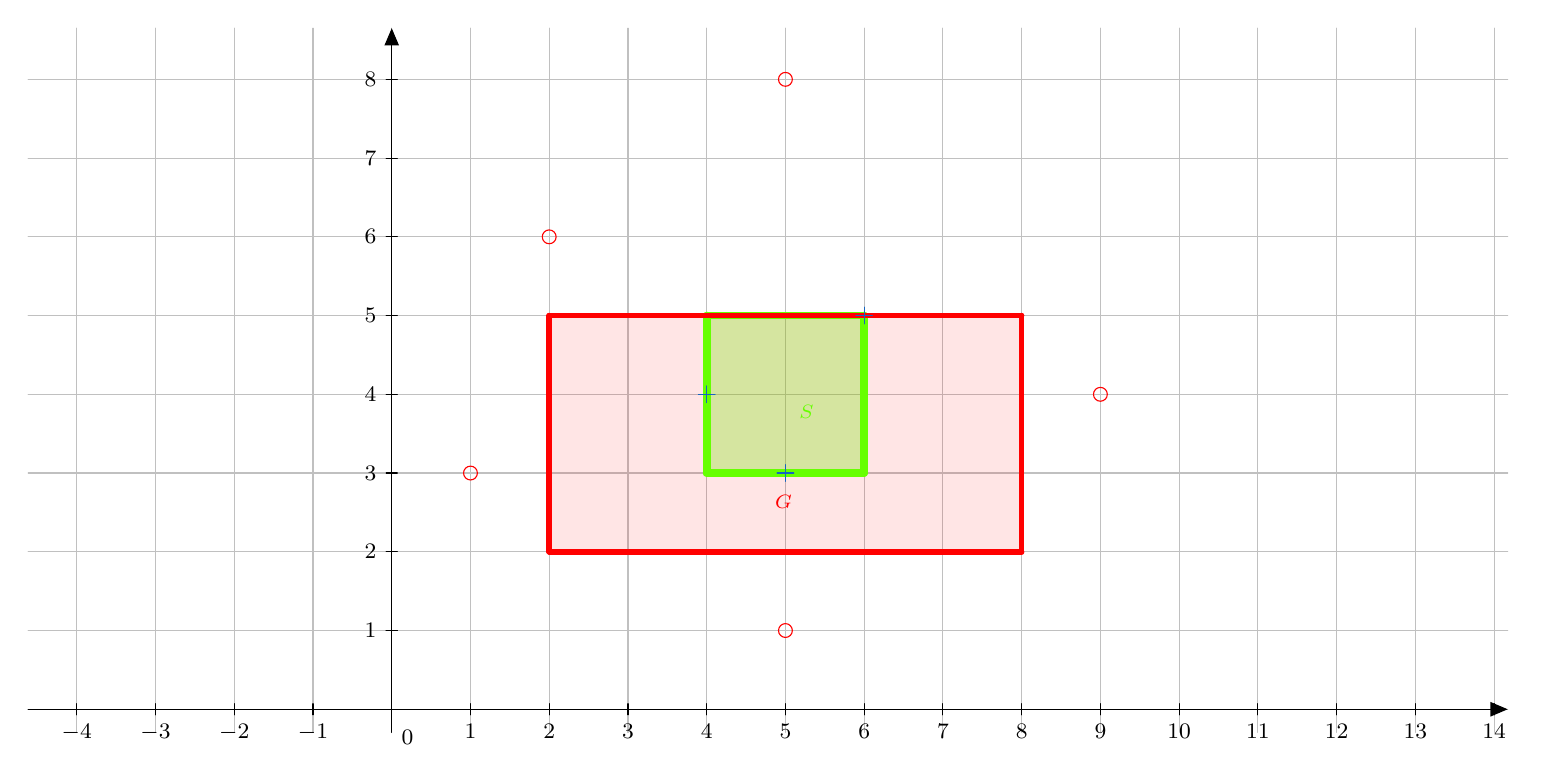
\begin{tikzpicture}[line cap=round,line join=round,>=triangle 45,x=1cm,y=1cm]\draw [color=cqcqcq,, xstep=1cm,ystep=1cm] (-4.616401981112383,-0.29433286572230233) grid (14.172797298127916,8.649275175241309);\draw[->,color=black] (-4.616401981112383,0) -- (14.172797298127916,0);\foreach \x in {-4,-3,-2,-1,1,2,3,4,5,6,7,8,9,10,11,12,13,14}\draw[shift={(\x,0)},color=black] (0pt,2pt) -- (0pt,-2pt) node[below] {\footnotesize $\x$};\draw[->,color=black] (0,-0.29433286572230233) -- (0,8.649275175241309);\foreach \y in {,1,2,3,4,5,6,7,8}\draw[shift={(0,\y)},color=black] (2pt,0pt) -- (-2pt,0pt) node[left] {\footnotesize $\y$};\draw[color=black] (0pt,-10pt) node[right] {\footnotesize $0$};\clip(-4.616401981112383,-0.29433286572230233) rectangle (14.172797298127916,8.649275175241309);\fill[line width=2.8pt,color=wwffqq,fill=wwffqq,fill opacity=0.3] (4,3) -- (6,3) -- (6,5) -- (4,5) -- cycle;\fill[line width=2pt,color=ffqqqq,fill=ffqqqq,fill opacity=0.1] (2,2) -- (8,2) -- (8,5) -- (2,5) -- cycle;\draw [line width=2.8pt,color=wwffqq] (4,3)-- (6,3);\draw [line width=2.8pt,color=wwffqq] (6,3)-- (6,5);\draw [line width=2.8pt,color=wwffqq] (6,5)-- (4,5);\draw [line width=2.8pt,color=wwffqq] (4,5)-- (4,3);\draw [line width=2pt,color=ffqqqq] (2,2)-- (8,2);\draw [line width=2pt,color=ffqqqq] (8,2)-- (8,5);\draw [line width=2pt,color=ffqqqq] (8,5)-- (2,5);\draw [line width=2pt,color=ffqqqq] (2,5)-- (2,2);\begin{scriptsize}\draw [color=ffqqqq] (5,1) circle (2.5pt);\draw [color=ffqqqq] (1,3) circle (2.5pt);\draw [color=ffqqqq] (2,6) circle (2.5pt);\draw [color=ffqqqq] (5,8) circle (2.5pt);\draw [color=ffqqqq] (9,4) circle (2.5pt);\draw [color=rvwvcq] (5,3)-- ++(-3pt,0 pt) -- ++(6pt,0 pt) ++(-3pt,-3pt) -- ++(0 pt,6pt);\draw [color=rvwvcq] (4,4)-- ++(-3pt,0 pt) -- ++(6pt,0 pt) ++(-3pt,-3pt) -- ++(0 pt,6pt);\draw [color=rvwvcq] (6,5)-- ++(-3pt,0 pt) -- ++(6pt,0 pt) ++(-3pt,-3pt) -- ++(0 pt,6pt);\draw[color=wwffqq] (5.267301223247963,3.7772955108811597) node {$S$};\draw[color=ffqqqq] (4.9751094832733,2.633936528371607) node {$G$};
\end{scriptsize}
\end{tikzpicture}